\chapter{Introduction}
\label{chapter:Introduction}
\thispagestyle{myheadings}

\section{Context and contents of this thesis}
\label{sec:history}

\indent Quantum Computing offers us powerful machines that offer a novel approach to processing new information based on the principles of Quantum Mechanics. By utilizing Quantum Mechanical principles, quantum computing allows to run new types of algorithms at fast and efficient speeds which can lead to breakthroughs in cryptography, machine learning, or drug discovery. In 1936, Alan Turing developed the model for a programmable computer which would be known as the \textit{Turing Machine} and later on developed the theory of the \textit{Universal Turing Machine} which can simulate any Turing Machine. If an algorithm can be performed on any piece of hardware, then there is an equivalent algorithm for the Universal Turning Machine which can perform the same exact same task 
\cite{PLMS:PLMS0230}.
This concept would give rise to the concept of Quantum Simulations. In 1982, Richard Feynmann suggested building computers based on the principles of Quantum Mechanics to avoid difficulties in solving two important difficult algorithms - Shor's Algorithm (finding prime factors of any integer and solving the discrete logarithm) and Grover's Algorithm (fast search algorithm on unstructured search space) 
\cite{Feynman1982}. \newline
\indent Current approaches to Quantum computation rely on the principles of superposition and entanglement for an edge over classical computing. There are several requirements for a physical implementation of a quantum computer such as a defined extendable qubit array for stable memory, feasible state preparation for the initial state, long decoherence time, a universal set of gate operations and capability for single quantum measurements \cite{Nielsen:2011:QCQ:1972505}. \newline
\indent One practical system to simulate via quantum computation are molecular systems.
Computational Chemistry aids in research and development in drug and materials discovery which require demanding computational tools and power. The inherent quantum nature of molecular systems make it an excellent candidate to test quantum computing on as well as provide accurate modeling to researchers. Many problems in computational chemistry exist such as prediction of chemical reactions and the description of excited electronic states, transition states, and ground states of transition metal complexes. Using current computational methods require computational resources that scale exponentially with the system size. The ability to tap into the properties of quantum entanglement and superposition will greatly help computational speed up as now we will be able to deal with multiple variables simultaneously with quicker computational time.\cite{aspuru-guzik_photonic_2012}. \newline
\indent 

\section{Structure of this thesis}
\label{sec:history}
\indent This structure is divided into $6$ chapters. The rest of this chapter will focus on the needed mathematical, scientific and notation knowledge of Quantum Mechanics, Quantum Computing, Linear Optical Quantum Computing, and Quantum Walks followed by the purpose of the entire thesis. Chapter 2 will provide a description on the Motivation of this work. Chapter 3 will provide a System Description describing the abstraction, software implementation, and experimental setup. Chapter 4 will define out the Optical Benzene System mathematically. Chapter 5 will discuss the analysis of the Eigenenergies and Eigenstates of the System and Chapter 6 will finally wrap things up. The Appendix will contain information on the conventional Benzene molecule and the Matrix Logarithm operation.



\section{Background}
\label{sec:history}
\subsection{Quantum Mechanics}
The language of Quantum Physics must first be understood to go about with any sort of work involving Quantum Algorithms or Quantum Chemistry and beyond. In this section, a brief introduction to the mathematical formalism and physical meaning behind Quantum Mechanics will be defined and given. A very powerful formalism to put Quantum Mechanics in a simplistic way is through Dirac Formalism which is very important to applications in Quantum Mechanics such as quantum information. The mathematics of Quantum Mechanics is described via Linear Algebra. Let us start with some important details:
\begin{enumerate}
    \item A vector will be denoted as $\ket{n}$ or $\bra{n}$ (More on this notations meeting later).
    \item Vectors are complex and thus can have imaginary components. 
    \item Vectors may have infinite components and have the possibility of having a continuum of components.
    \item The state of a system is described by a vector
    \item Observables (measurable things) correspond to operators which perform a linear transformations on vectors.
    \item The principle of a superposition allows for the linear combination of two wavefunctions to be a possible wavefunction for the system.
\end{enumerate}
\newline
%%%%%%%%%%%%%%%%%%%%%
\textbf{Dirac Notation}\newline
A vector or state will be denoted as $\ket{\psi}$ which is known as the "ket"-vector or as a "bra"-vector denoted as $\bra{\psi}$ (Note that the bra is the complex conjugate transpose of the ket). A bra and ket together together provides a braket $\braket{n|m}$ which denotes the scalar (inner) product of the vectors $\ket{n}$ and $\ket{m}$ (Note that $\braket{n|m} = \braket{m|n}^{*}$). \newline
%%%%%%%%%%%%%%%%
\textbf{Vector Space} \newline
The vector space contains scalars and vectors. One can define a new state $\psi$ with the superposition of some states $\alpha$ and $\beta$ multiplied by scalar constants $a, b$ respectively:
\begin{equation}
    \ket{\psi} = a\ket{\alpha} + b \ket{\beta}
\end{equation}
$a$ and $b$ must follow the normalization property of Probability Theory: 
\begin{equation}
    |a|^2 + |b|^2 = 1
\end{equation}
A vector may also be expanded as a set of linearly independent basis vectors $\ket{e_{i}}, i = 1,2,..,n$:
\begin{equation}
    \ket{\alpha} = \sum_{i=1}^{n} a_{i} \ket{e_{i}}
\end{equation}
Where $a_{i}$ are complex scalars and denoted as the components of the vector and $n$ to be the dimension of the vector space. 
If we describe $e_{i}$ to be an orthonormal basis:
\begin{equation}
    \braket{e_{i}|e_{j}} = \delta_{i,j}
\end{equation} 
The components of the vector $\ket{\alpha}$ are given by:
\begin{equation}
    a_{i} = \braket{e_{i}|\alpha}
\end{equation}
And the inner product of $\alpha$ and $\beta$ are given by:
\begin{equation}
    \braket{\alpha|\beta} = \sum_{i=1}^{n} a_{i}^{*}b_{i}
\end{equation}
And the norm of the vector $\alpha$ is given by:
\begin{equation}
    \braket{\alpha|\alpha} = \sum_{i=1}^{n} a_{i}^{*}a_{i}
\end{equation}
%%%%%%%%%%%%%
\textbf{Linear Transformations/Operators} \newline
An Operator $\hat{O}$ will apply an linear transformation to a vector $\ket{\alpha}$ to get a new transformed vector $\ket{\alpha'} = \hat{O}\ket{\alpha}$ and obeys linearity conditions:
\begin{equation}
    \hat{O}( a\ket{\alpha} + b \ket{\beta}) = a \hat{O}\ket{\alpha} + b \hat{O}\ket{\beta}
\end{equation}
The action of an operator $\hat{O}$ on an arbitrary vector can be obtained from the action on the basis states which will now be denoted as $\ket{i}$:
\begin{equation}
    \hat{O}\ket{j} = \sum_{i=1}^{n} O_{ij}\ket{i}
\end{equation}
\begin{equation}
    O_{ij} = \braket{i|\hat{O}|j}
\end{equation}
$O_{ij}$ is known as the component or matrix element of the operator $\hat{O}$ which forms a $n \times n$ matrix. \newline
%%%%%%%%%%%%%%%%%
\textbf{Hermitian Transformations} \newline
If $\hat{O}$ is an operator, then the hermitian conjugate operator $\hat{O}^{\dagger}$ is given by:
\begin{equation}
    \braket{\alpha|\hat{O}^{\dagger}|\beta} = \braket{\beta|\hat{O}|\alpha}^{*}
\end{equation}
A very important concept in Quantum mechanics involve Hermitian Conjugates equal the operator of itself:
\begin{equation}
    \hat{O} = \hat{O}^{\dagger}
\end{equation}
These operators are said to be \textit{hermitian} \newline
\textbf{Eigenvalues/Eigenvectors} \newline
Eigenvalue/Eigenvector problems show up all throughout Quantum Mechanics:
\begin{equation}
    \hat{O}\ket{n} = \lambda \ket{n}
\end{equation}
Where $\lambda$ is the eigenvalue of the system and the vector $\ket{n}$ represent the eigenstates/eigenvectors of the system. \newline
If a operator $\hat{O}$ is hermitian, the following properties hold:
\begin{enumerate}
    \item All eigenvalues are real 
    \item Eigenvectors corresponding to different eigenvalues are orthongonal 
    \item The eigenvectors span the vector space
\end{enumerate}
The Operator Identity which is very useful due to its ability to be inserted anywhere is as follows: 
\begin{equation}
    I = \sum_{i=1}^{n} \ket{i}\bra{i}
\end{equation}
Using this identity operator, we can derive the components of a operator $\hat{O}$ in the basis \{$\ket{i}$\} as the following:
\begin{equation}
    \hat{O} = \hat{I} \cdot \hat{O} \cdot \hat{I} = \sum_{i,j} \ket{i}\braket{i|\hat{O}|j}\bra{j} = \sum_{i,j} \ket{i}O_{ij}\bra{j}
\end{equation}
%%%%%%%%%%%%%%%%%%%
\textbf{Time Evolution/Unitary Transformations} \newline
Often for experiments and simulations, one would like develop an eigenfunction expansion to provide the means to seeing the time evolution of a wavestate/wavefunction $\ket{\psi}$. One may move a state forward in time by applying a time evolution operator. Where the state as a function of time after applying the time-evolution operator is given by:
\begin{equation}
    \ket{\psi (t)} = \hat{U}\ket{\psi(0)}
\end{equation}
Where the time operator $\hat{U}$ is defined as 
\begin{equation}
    \hat{U} = e^{-i \hat{H}t/\hbar}
\end{equation}
Applying the Identity operator on the time evolved state and defining $\ket{i}$ as the eigenstates of the Hamiltonian $\hat{H}$ we obtain the following expression:
\begin{equation}
    \ket{\psi (t)} = e^{-i\hat{H}t/\hbar} \sum_{i} \ket{i}\braket{i|\psi(0)} = \sum_{i} \ket{i}\braket{i|\psi(0)}e^{-iE_{i}t/\hbar}
\end{equation}
The time evolution operator is known as a \textit{Unitary operator}. Unitary operators are defined as transformations which preserve the scalar product:
\begin{equation}
    \braket{\phi|\psi} = \braket{\hat{U}\phi|\hat{U}\psi} = \braket{\phi|\hat{U}^{\dagger}\hat{U}\psi} = \braket{\phi|\psi} \rightarrow \hat{U}\hat{U}^{\dagger} = I
\end{equation}
%%%%%%%%%%%%%%%%%%%%%%%%%%%%%%%%%%%%%%
\textbf{Change of Basis} \newline
Change of basis under Dirac Formalism is useful when redefining states or making the matrix of a system simpler in a QM setup. Once again the Identity Operator will come in handy for making this setup. \newline
Let $\ket{a_{i}}$ and $\ket{b_{i}}$ ($i = 1,2,...,n$) be two sets of normalized basis vectors. Two resolutions will fall out of the identity operator: 
\begin{equation}
    \hat{I} = \sum_{i} \ket{a_{i}}\bra{a_{i}} = \sum_{i} \ket{b_{i}}\bra{b_{i}}
\end{equation}
Now we derive a relation that relates two vector sets:
\begin{equation}
    \ket{a_{i}} = \sum_{j} \ket{b_{j}}\braket{b_{j}|a_{i}}
\end{equation}
A vector $\ket{\psi}$ can be expanded as:
\begin{equation}
    \ket{\psi} = \sum_{i} \ket{a_{i}}\braket{a_{i}|\psi} = \sum_{i} \ket{b_{i}}\braket{b_{i}|\psi}
\end{equation}
With components related as: 
\begin{equation}
    \braket{a_{i}|\psi} = \sum_{j} \braket{a_{i}|b_{j}}\braket{b_{j}|\psi}
\end{equation}
We can rewrite this in matrix notation as: 
\begin{equation}
    {\psi}^{(a)} = \textbf{S}\psi^{(b)}
\end{equation}
Where $\psi^{a/b}$ is the vector with elements $\braket{a_{i}/b_{i}|\psi}$ and the matrix $\textbf{S}$ with elements $S_{ij} = \braket{a_{i}|b_{j}}$ \newline
For an operator $\hat{O}$ we get the following expression: 
\begin{equation}
    \braket{a_{i}|\hat{O}|a_{j}} = \sum_{k,m} \braket{a_{i}|b_{k}} \braket{b_{k}|\hat{O}|{b_{m}}}\braket{b_{m}|a_{i}}
\end{equation}
In matrix notation the above epxression becomes:
\begin{equation}
    \textit{\textbf{O}}^{(a)} = \textbf{\textit{S}}\textit{\textbf{O}}^{(b)}\textbf{\textit{S}}^{-1}
\end{equation}
Where $\textbf{\textit{S}}^{-1}$ has components $S_{ij}^{-1} = \braket{b_{i}|a_{j}}$. This transformation allows for the diagonalization of the matrix $\textit{\textbf{O}}^{(b)}$ by finding a transformation matrix $\textbf{\textit{S}}$ such that $\textit{\textbf{O}}^{(a)}$ is diagonal is equivalent to transforming a basis consisting of the eigenvectors of an operator $\hat{O}$. \newline
%%%%%%%%%%%%%%%%%%%%%%%%%%%%%%%%%%%%%%%%%%%%%%%%
\textbf{Statistical Interpretation} \newline
A quantum mechanical system is described by a vector $\ket{\psi}$ in a Hilbert space $\mathcal{H}$ where every vector in $\mathcal{H}$ describes a possible state for the system. \newline
Every observable (measurable quantity) $A$ corresponds to a hermitian operator $\hat{A}$ acting on the vectors in $\mathcal{H}$. \newline
The expectation value for an observable $A$ is 
\begin{equation}
    \braket{A} = \frac{\braket{\psi|\hat{A}|\psi}}{\braket{\psi|\psi}} = \braket{\psi|\hat{A}|\psi}
\end{equation}
A measurement of an observable $A$ gives one of the eigenvalues $\lambda_{i}$ of the hermitian operator $\hat{A}$ with eigenvectors $\ket{n_{i}}$. \newline 
Given $\ket{\psi}  = \sum_{i} \ket{n_{i}}\braket{n_{i}|\psi}$, then the probability $P_{i}$ to get $\lambda_{i}$ after a measurement is given by: 
\begin{equation}
    P_{i} = \frac{|\braket{n_{i}|\psi}|^2}{\braket{\psi|\psi}} = |\braket{n_{i}|\psi}|^2
\end{equation}
Note the normalization $\braket{\psi|\psi} = 1$. \newline
After measurement, the wavefunction collapses into the eigenstate/eigenvector $\ket{n_{i}}$ corresponding to the measured eigenvalue $\lambda_{i}$.
Repeated measurement of $A$ after this measurement will keep giving the same measurement $\lambda_{i}$ with probability $1$. \newline
%%%%%%%%%%%%%%%%%%%%%%%%%
\textbf{Ladder Operators} \newline
In the context of Linear Algebra but specifically Quantum Mechanics, ladder operators are operators (matrices) that can increase or decrease the eigenvalue of another operator or state. There are two types of ladder operators - the raising operator (or creation operator) and the lowering operator (annihilation or destruction operator). They are frequently used in Quantum Mechanics , especially in the harmonic oscillator systems, quantum optical systems, and angular momentum. \newline
Suppose you have two operators $N$ and $A$ and a constant $\gamma$ with the following commutation relation:
\begin{equation}
    [N, A] = \gamma A
\end{equation}
Operator $N$ has an eigenstate $\ket{n}$ with eigenvalue $n$ that satisfies the eigenvalue-eigenvector problem:
\begin{equation}
    N\ket{n} = n \ket{n}
\end{equation}
Then the operator $A$ acts on the eigenstate $\ket{n}$ such that the eigenvalue is shifted by the constant scalar $\gamma$ 
\begin{eqnarray}
NA\ket{n} = (AN + [N,A])\ket{n} \\
= AN\ket{n} + [N,A]\ket{n} \\
= An\ket{n} + \gamma A\ket{n} \\
 = (n + \gamma) A \ket{n} 
\end{eqnarray}
Therefore, since $\ket{n}$ is an eigenstate of $N$ then $A\ket{n}$ is an eigenstate of $N$ with an eigenvalue of $n + \gamma$. In other words, the operator $A$ is a raising operator if $\gamma$ is real and positive and a lowering operator if $\gamma$ is is real and negative. \newline
Let us define some basic raising and lowering operators (2D) in their matrix representation and defined in terms of the pauli matrices which are as follows: 
\begin{equation}
    \sigma_{1} = \sigma_{x} =  \begin{pmatrix} 0 & 1 \\ 1 & 0 \end{pmatrix} ,
    \sigma_{2} = \sigma_{y} = \begin{pmatrix} 0 & -i \\ i & 0 \end{pmatrix} ,
    \sigma_{3} = \sigma_{z} = \begin{pmatrix} 1 & 0 \\ 0 & -1 \end{pmatrix} 
\end{equation}
The raising (creation) operator: 
\begin{equation}
    a^{\dagger} = a_{+} = \begin{pmatrix} 0 & 0 \\ 1 & 0 \end{pmatrix} = \frac{1}{2}(\sigma_{1} - i\sigma_{2})
\end{equation}
The lowering (annihilation or destruction) operator:
\begin{equation}
    a = a_{-} = \begin{pmatrix} 0 & 1 \\ 0 & 0 \end{pmatrix}  = \frac{1}{2}(\sigma_{1} + i\sigma_{2})
\end{equation}
The number operator (particle or one) operator:
\begin{equation}
    n = \begin{pmatrix}  0 & 0 \\ 0 & 1 \end{pmatrix} = a^{\dagger}a = \frac{1}{2}(1 - \sigma_{3})
\end{equation}
The other number operator (hole or zero) operator:
\begin{equation}
    h = \bar{n} = \begin{pmatrix} 1 & 0 \\ 0 & 0 \end{pmatrix} = aa^{\dagger} = \frac{1}{2} ( 1 + \sigma_{3})
\end{equation}
The number operators follow the following anticommutation relation algebraically (produces the identity operator): 
\begin{eqnarray}
a^{\dagger}a + aa^{\dagger} = n + h = \textbf{1}
\end{eqnarray}
%%%%%%%%%%%%%%%%%%%%%%%%%%%%%%%%%%%%%%%%%%%%%%%%%%%%%%%%%%%%%%%%%%%%%%%%%%%%%%%%%%%%%
\subsection{Quantum Optics}
Quantum optics is an area of physics that encompasses Quantum Mechanics, Electromagnetic Theory, and Photonics in order to investigate the phenomena involving light and its interaction with matter such as atoms and molecules. In the context of this thesis and further work it is important to understand the quantum mechanical behavior of optical equipment such as beam splitters which split incident light into two or more beams. \newline
\textbf{Quantum Mechanical Description of Beam Splitters} \newline
Beam splitters are important in quantum mechanics, especially in quantum information where beam splitters are important for teleportation, bell measurements, and entanglement. \newline
Suppose you have two electric fields $E_{1}$ and $E_{2}$ enter the beam splitter at separate ports respectively. The first field evolves with the following relation: $E_{1} \rightarrow tE_3 + rE_4$ and the second field evolves with the the following relation: $E_2 \rightarrow rE_3 + tE_4$ where $t,r$ are the transmission and reflection coefficients for the beam splitter. \newline \newline
Assuming the beamsplitter is lossless or approximately lossless, it can be deduced that the transformation undergone in the relations above is unitary which gives rise to the following relations
\begin{equation}
    |t|^2 + |r|^2 = 1
\end{equation}
\begin{equation}
    r^{*}t + rt^{*} = 0
\end{equation} 
Now represent the fields as raising and lowering operators. Let the two input fields be denoted by the lowering operators $a_{0} , a_{1}$ and the two output fields be denoted by the lowering operators $a_{2}$ and $a_{3}$ \cite{gerry2005introductory}. The transformation matrix of this relation is denoted below:
\begin{equation}
    \begin{pmatrix} a_{2} \\ a_{3} \end{pmatrix} = \begin{pmatrix} t' & r \\ r' & t \end{pmatrix} 
    \begin{pmatrix} a_{0} \\ a_{1} \end{pmatrix}
\end{equation}
The transformation matrix above must obey the following commutation relations: 
\begin{eqnarray}
[a_{i}, a_{j}^{\dagger}] = \delta_{ij} \\ {[a_{i}, a_{j}]} = 0 
\end{eqnarray}
The matrix must also follow Eq. (1.41) and Eq. (1.42) and $|r'| = |r|$ and $|t'| = |t|$. \newline
Utilizing a 50-50 beam splitter, the reflected and transmitted light is offset by a phase of $e^{\pm i \pi / 2} = \pm i$. Which gives rise to the following relations for the output lowering operators.
\begin{equation}
    a_2 = \frac{1}{\sqrt{2}} (a_0 + ia_1), a_3 = \frac{1}{\sqrt{2}}(ia_0 + a_1)
\end{equation}
This transformation matrix can be represented as a unitary transformation given as
\begin{equation}
    \hat{U} = e^{i\frac{\pi}{4}(a_{0}^{\dagger}a_1 + a_{0}a_{1}^{\dagger})}
\end{equation}
\begin{equation}
    \begin{pmatrix} a_{2} \\ a_{3} \end{pmatrix} = \hat{U}^{\dagger} \begin{pmatrix} a_{0} \\ a_{1} \end{pmatrix} \hat{U}
\end{equation} \newline
%%%%%%%%%%%%%%%%%%%%%%%%%%%%%%%%%%%%%%
\subsection{Quantum Information/Computing}
\textbf{Introduction to Quantum Computing} \newline
Classical computers are built upon the concept of a \textit{bit}. Quantum computation and information are build upon the \textit{qubit} (quantum bit) the analog to the classical bit. The two possible states are based on the computational basis states of $\ket{0}$ and $\ket{1}$. As opposed to classical bits where a bit can either take a $0$ or $1$, a qubit can take another state formed from a superposition of states given as:
\begin{equation}
    \ket{\psi} = \alpha \ket{0} + \beta \ket{1}
\end{equation}
Where $\alpha$ , $\beta$ are complex numbers. When a qubit is measured, one will either get the state $\ket{0}$ with probability $|\alpha|^2$ or state $\ket{1}$ with probability $|\beta|^2$ , (Note the constants must follow the normalization condition $|\alpha|^2 + |\beta|^2 = 1$, as the sum of the probabilities must add up to $1$). Generally, the state of a qubit can be described as a unit vector in two-dimensional complex vector space. \newline
There are many physical ways to realize qubits such as:
\begin{enumerate}
    \item Two different polarizations of a photon
    \item Alignment of Nuclear Spin in a uniform magnetic field
    \item Two states of an electron orbiting a single atom. 
\end{enumerate}
A useful geometric representation of the qubit can be that of a spinor:
\begin{equation}
    \ket{\psi} = e^{i\gamma} \Big( \cos \frac{\theta}{2} \ket{0} + e^{i\varphi} \sin \frac{\theta}{2} \ket{1} \Big)
\end{equation}
Where $\theta, \varphi, \gamma$ are real numbers. The relative phase $\gamma$ doesn't give any observable effects so it can be neglected and the state can be boiled down to: 
\begin{equation}
   \ket{\psi} =  cos \frac{\theta}{2} \ket{0} + e^{i\varphi} \sin \frac{\theta}{2} \ket{1}. 
\end{equation}
The state of a single qubit can be visualized by the three-dimensional space of a Bloch Sphere (shown below). Note there is no generalization for a Bloch sphere for multiple qubits. 
\begin{figure}[htb]
    \centering
    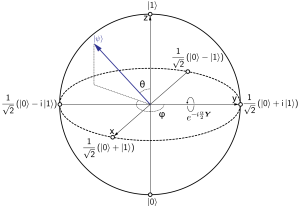
\includegraphics{1_Intro/Figures/bloch_sphere.png}
    \caption{Bloch sphere representation of a qubit}
    \label{fig:my_label}
\end{figure}
If there were two qubits, then a four computational basis is form of the states $\ket{00}, \ket{01}, \ket{10}, \ket{11}$. The state vector representing a possible superposition of these four states is given by: 
\begin{equation}
    \ket{\psi} = \alpha \ket{00} + \beta \ket{01} + \xi \ket{10} + \eta \ket{11}
\end{equation}
For a two qubit system, one can measure a subset of qubits, and so the probability of finding say just the first qubit gives $0$ with probability $|\alpha|^2 + |\beta|^2$, providing a post measurement state of:
\begin{equation}
    \ket{\psi '} = \frac{\alpha \ket{00} + \beta \ket{01}}{\sqrt{|\alpha|^2 + |\beta|^2}}
\end{equation}
The Bell state (EPR Pair) will be useful in Quantum Information especially for concepts like teleportation and superdense coding: 
\begin{equation}
    \frac{\ket{00}+ \ket{11}}{\sqrt{2}}
\end{equation}
%%%%%%%%%%%%%%%%%%%%%%%%%%%%%%
\textbf{Quantum Gates} \newline
In order to do qubit operations, the quantum analogue for classical wires and logic gates are needed to transport information and manipulate information. For example the NOT Gate which flips a bit into the opposite, would do the following operation on a qubit in the quantum analogue: 
\begin{equation}
    \alpha \ket{0} + \beta \ket{1} \rightarrow \alpha \ket{1} + \beta \ket{0}
\end{equation}
One can define several gate operations out of the pauli spin matrices $\{ \sigma_{x}, \sigma_{y}, \sigma_{z} \}$. For example the quantum NOT gate can be made out of the $\sigma_{x}$ matrix defined as the matrix $X$, Note that quantum gates require the constraint of that they must be unitary ($A^{\dagger}A = I$): 

\begin{equation}
    X = \begin{bmatrix} 
    0 & 1 \\
    1 & 0 \end{bmatrix}
\end{equation}
The $Z$ gate only acts on flipping the sign of the $\ket{1}$ state to $-\ket{1}$ , leaving $\ket{0}$ unchanged is given as the $\sigma_{z}$ matrix: 
\begin{equation}
    Z = \begin{bmatrix}
    1 & 0 \\
    0 & -1 \end{bmatrix}
\end{equation} 
Another important gate operation is the Hadamard gate also known as the \textit{square root of NOT} gate. The Hadamard Gate turns a $\ket{0}$ into $(\ket{0} + \ket{1})/\sqrt{2}$ and turns $\ket{1}$ into $(\ket{0} - \ket{1})/\sqrt{2}$ . (Note applying a Hadamard gate twice to a state does nothing to it as $H^2 = I$: 
\begin{equation}
    H = \frac{1}{\sqrt{2}}
    \begin{bmatrix}
    1 & 1 \\
    1 & -1 \end{bmatrix}
\end{equation}
In the bloch sphere representation, the hadamard operation would correspond to rotations around the different axes which in this case causes $180$ degree rotation around $x$ and a $90$ degree rotation around $y$. \newline
Other Single Qubit Operation gates include the $Y$-gate, Phase Gate $S$, and $\pi / 8$ gate $T$ given as the following:
\begin{equation}
    Y = 
    \begin{bmatrix}
    0 & -i \\
    i & 0 
    \end{bmatrix}
    , 
    S = 
    \begin{bmatrix}
    1 & 0 \\
    0 & i 
    \end{bmatrix}
    ,
    T = 
    \begin{bmatrix}
    1 & 0 \\
    0 & e^{i\pi/4}
    \end{bmatrix}
\end{equation}
The next important computing operation is of Controlled operations such as "If this then do that". The controlled-NOT gate or CNOT for short is a quantum gate with two input qubits, known as the \textit{control} qubit and \textit{target} qubit. The CNOT operation is given by $\ket{c}\ket{t} \rightarrow \ket{c} \ket{t \oplus c}$. For example, if the control qubit is set to $\ket{1}$ then the target qubit is flipped, otherwise the target qubit is left alone. The matrix representation of CNOT is given by: 
\begin{equation}
    CNOT = 
    \begin{bmatrix}
    1 & 0 & 0 & 0 \\
    0 & 1 & 0 & 0 \\
    0 & 0 & 0 & 1 \\
    0 & 0 & 1 & 0
    \end{bmatrix}
\end{equation}
Next in the context of this thesis, we will discuss the Linear Optical Quantum Computing. 
%%%%%%%%%%%%%%%%%%%%%%%%%%%%%%%%%%%%%%%%%%%%%%%%
\subsection{Linear Optical Quantum Computing} \newline
\textbf{Introduction to LOQC} \newline
Quantum Computing via Linear Optics has the edge that photons which can be used for quantum information storage is potentially free from decoherence as the information in a photon tends to stay where it is; however, the problem of photons being unable to interact with each other which makes it difficult to apply gate operations. In order to create an optical quantum computer, one must come up with a way to introduce interaction between photons \cite{RevModPhys.79.135}. For example, one may introduce large cross-Kerr nonlinearities to induce a single photon CNOT operation. Another method is making projective measurements with photo-detectors; however, optical quantum gates are probabilistic (currently due to this nature, the gate can fail and destroy information in the computation). \newline
The building blocks of linear optics include beam splitters, half wave plates, quarter wave plates, phase shifters, and other optical equipment. Building a network of these optical components will suffice a universal quantum computing systems; however, the size of such a network grows rapidly. \newline
%%%%%%%%%%%%%%%%%%%%%%%%%%%%%%%%%%
\textbf{Linear Optical Multiports} \newline
Multiports are a generalization of a optical device made out of beam splitters and phase shifters. In the case of LOQC, bosonic qubits are utilized which are defined by the states of optical modes known as Fock states. Using the basis for a Quantum Harmonic Oscillator and electromagnetic field quantization, define the well known raising and lowering operators: 
\begin{equation}
    a\ket{n} = \sqrt{n} \ket{n-1}
\end{equation}
\begin{equation}
    a^{\dagger} \ket{n} = \sqrt{n+1} \ket{n+1}
\end{equation}
$n$ refers to the number of photons in a mode and we assert the condition of $a\ket{0} = 0$ due to no eigenstate of lower energy than the ground state. In order to generate a Fock state of the $k$th mode $\ket{n_k}$ from the vacuum, apply the ladder operators several times.
\begin{equation}
    \ket{n_k} = \frac{a_{k}^{\dagger}}{\sqrt{n_{k}!}}\ket{0}
\end{equation}
Given a linear quantum gate with $N$ inputs, one may describe the model classically as a relation between outgoing and incoming waves \cite{10.1007/3-540-49208-9_36}.
\begin{equation}
    b_{i} = \sum_{j=1}^{N} \Lambda_{ij}q_{j}
\end{equation}
where $b_{i}(q_{i})$ are the complex amplitudes of the outgoing (incoming) waves and $\Lambda_{ij}$ is the unitary matrix transformation from port $i$ to port $j$ which depends on the chosen linear optical element
\begin{figure}[H]
    \centering
\begin{tikzpicture}[
node distance = 4mm and 22mm
                        ]
\node (adc) [draw,minimum size=24mm] {$\hat{\Lambda}$};
%
\coordinate[above left = of adc.west]   (a1);
\coordinate[below = of a1]              (a2);
\coordinate[below = of a2]              (a3);
\coordinate[above right= 4mm and 22mm of adc.east]  (b1);
\foreach \i [count=\xi from 1] in {2,...,3} 
    \coordinate[below=of b\xi]  (b\i);
%
\foreach \i [count=\xi from 1] in {$q_{3}$,$q_{2}$,$q_{1}$}
\draw[-latex']  (a\xi) node[left] {\i} -- (a\xi-| adc.west);
\foreach \i [count=\xi from 1] in {$b_{3}$,$b_{2}$,$b_{1}$}
    \draw[-latex'] (adc.east |- b\xi) -- (b\xi) node[right] {\i};
\end{tikzpicture}
    \caption{Linear Quantum Gate with $N$ input and output ports ($N=3$ in figure)}
    \label{fig:my_label}
\end{figure}
Quantum mechanically, $q_{i}$ and $b_{i}$ become operators that satisfy the commutation relations in Eq. (1.44) and Eq. (1.45). Given $N$ input ports, the basis can be defined as a product of number states for each mode: 
\begin{equation}
    \ket{n_{N}}\otimes \dots \otimes \ket{n_2} \ket{n_1} = \ket{n_{N}\dots n_{2}n_{1}}
\end{equation}
It is impossible to know the path taken by a photon within a multiport device, one must add up all the accumulated phases over all the paths inside the system and then add the probability amplitudes of all the possibilities. This results in a superposition given by the state $\ket{m_{N} \dots m_{2} m_{1}}$ after the transformation $Lambda$ is performed. Assume that the system is lossless then the number of photons is preserved during the entire transformation. \newline
Under the Heisenberg picture (quantum mechanical representation where time dependence is absorbed into the operator while keeping the basis fixed), the operators $q_{i}$ and $b_{i}$ evolve as:
\begin{eqnarray}
q_{i}^{\dagger} \rightarrow b_{i}^{\dagger} = \sum_{k=1}^{N} \Lambda_{ik}^{*}q_{k}^{\dagger} = U^{\dagger}q_{i}^{\dagger}U \\
q_{i} \rightarrow b_{i} = \sum_{k=1}^{N} \Lambda_{ik}q_{k} = U^{\dagger}q_{i}U
\end{eqnarray}
Given that $\Lambda$ is unitary, Eq.(1.66) can be rewritten:
\begin{equation}
    Uq_{i}^{\dagger}U^{\dagger} = \sum_{k=1}^{N} \Lambda_{ki}q_{k}^{\dagger}
\end{equation}
The number state when given an arbitrary input for the $N$th mode can be generalized to:
\begin{equation}
    \ket{n_{N} \dots n_{2}n_{1}} = \frac{a_{N}^{\dagger n_{N}}\dots a_{2}^{\dagger n_{2}}a_{1}^{\dagger n_{1}}}{\sqrt{n_{N}!\dots n_{2}!n_{1}!}} \ket{0\dots0}
\end{equation}
In order to find the exit state, the number state is operated on with $U$ multiple times and keep in mind of the following property:
\begin{equation}
    Uq_{i}^{\dagger 2} = Uq_{i}^{\dagger}Iq_{i}^{\dagger}I = Uq_{i}^{\dagger}U^{\dagger}Uq_{i}^{\dagger}U = (Uq_{i}^{\dagger}U^{\dagger})^{2}U
\end{equation}
\begin{eqnarray}
U\ket{n_{N} \dots n_{2}n_{1}} = \frac{(Uq_{N}^{\dagger}U^{\dagger})^{n_{N}} \dots (Uq_{2}^{\dagger}U^{\dagger})^{n_{2}}(Uq_{1}^{\dagger}U^{\dagger})^{n_{1}}}{\sqrt{n_{N}!\dots n_{2}!n_{1}!}} U \ket{0\dots0} \\
 = \frac{\prod_{k=1}^{N} (\sum_{l=1}^{N} \Lambda_{lk} q_{l}^{\dagger})^{n_{k}}}{\sqrt{n_{N}!\dots n_{2}!n_{1}!}} \ket{0 \dots 0}
\end{eqnarray}
%%%%%%%%%%%%%%%%%%%%%%%%%%%%%%%%%%%%%%%
\subsection{Quantum Walks}
\textbf{Introduction} \newline
Much of the background in this section is attributed to Dr. Kempe on his explanation of the concept of Quantum Random Walks in the journal \textit{Contemporary Physics }\cite{doi:10.1080/00107151031000110776}. \newline
\indent A random walk is a stochoastic or random process that describes a path that consists of succession of random steps on a mathematical space. In the relevant application of Computational Chemistry, this could be the path traced by a molecule or an electron or a photon as it travels in a liquid or gas or around a molecule. Quantum walks are the quantum analogue of a classical random walk \cite{PhysRevA.48.1687}. One must be careful to use the phrase \textit{quantum random walk} because even though a measurement is random, the \textit{evolution} of the state after the walk itself is not random but \textit{unitary} compared to a classical random walk where the evolution of the walk is random based on a defined mathematical space \cite{https://open.bu.edu/handle/2144/23564}. \newline
\indent The main idea behind quantum random walks is to iterate the walk by repeating the succession of some unitary translation $U$ and rotation $R(\theta)$ without the needed measurement $M_{z}$ at intermediate time steps. Additionally, the position space of the particle must be discretized into a finite space such as a lattice or a graph. Quantum computers function with discrete registers where the Hilbert space is large but finite. A quantum computer should be able to simulate a quantum walk efficiently and use the simulation to solve computational problems which leads to uncovering efficient and fast algorithms. In principle any quantum algorithm can be simulated by a quantum walk. A multi-particle quantum walk (involving interacting many-body systems) may be used as an architecture for building a scalable quantum computer without the need for time-dependent control \cite{Childs791}. \newline 
\indent Before looking at the structure of quantum walks, let us visit Classical Discrete Random Walks, particularly those on a line with a particle jumping either left or right. For example, if we have a lattice with $N$ nodes with each node having $6$ vertices and the outcome of the particles moment is dependent on a dice roll described by a stochastic process $\{Z_{n}\}$. We can describe the probability of going to the right as $p$ and to the left as $1-p$. We may describe each step by a Bernoulli-distributed random variable where the probability of finding the particle in position $k$ after $n$ steps and having an initial position $Z_{0}=0$ is given by the binomial distribution:
\begin{equation}
    T_{n} = \sum_{k=1}^{n} Y_{i} = \frac{1}{2}(Z_{n} + n)
 \end{equation}
 \begin{equation}
     P(Z_{n} = k | Z_{0} = 0) = 
     \begin{cases}
     \binom{n}{\frac{1}{2}(k+n)} p^{\frac{1}{2}(k+n)}q^{\frac{1}{2}(n-k)}, & \frac{1}{2}(k+n) \in \mathbb{N} \cup \{0\}; \\
     0, \text{otherwise} 
     \end{cases}
 \end{equation}
  \begin{figure}[H]
     \centering
     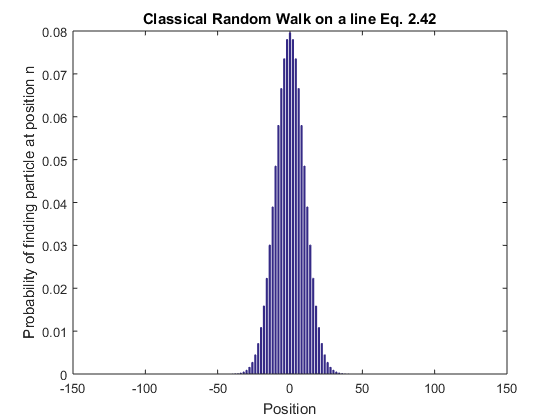
\includegraphics[scale=0.6]{1_Intro/Figures/classical_walk.png}
     \caption{MATLAB Plot of Eq. 1.74 for $n = 100, p = \frac{1}{2}$. The probability of finding the particile at position $k = 0$ is equal $0.0795$.}
     \label{fig:my_label}
 \end{figure}
 The structure of quantum walks can be built up and understood from the example of a \textit{discrete time quantum walk} (DTQW). This sort of DTQW which will be shown is of a coined DTQW which consists of the following components - a walker, a coin, and a set of observables \cite{Venegas-Andraca2012}. The walker will consist of a infinite dimensional space Hilbert space $\mathcal{H}_{p}$ with a quantum system. Position states $\ket{n}$ will be in this Hilbert space with $\ket{i}_{p}$ basis states spanning the space as well. The walker will be initialized at the origin: $\ket{n}_{initial}=\ket{0}_{p}$. The coin will be a quantum system within a two-dimensional hilbert space $\mathcal{H}_{c}$ , and thus will take states of either $\ket{0}$ or $\ket{1}$. The state $\ket{c} \in \mathcal{H}_{c}$ with a generalized expression in the form of $\ket{c} = a\ket{0}_{c} + b \ket{1}_{c}$. \newline
\indent The total state of the quantum walk will reside in the total Hilbert Space: $\mathcal{H}_{t} = \mathcal{H}_{p} \otimes \mathcal{H}_{c}$. Next part of the process is to define an evolution operator to be applied to the coin state following by a conditional shift operator to the total quantum system. The coin operator will put the coin state into a superposition and then randomness is introduced by performing an measurement on the system after the two evolution operators are applied several times. We define the coin operation $\Hat{C}$, the \textit{Hadamard Operator} to apply a unitary rotation on the coin basis: 
\begin{equation}
    \Hat{H} = \frac{1}{\sqrt{2}} (\ket{0}_{c}\bra{0} + \ket{0}_{c}\bra{1} + \ket{1}_{c}\bra{0} - \ket{1}_{c}\bra{1})
\end{equation}
Next, the \textit{conditional translation} is applied to a position state (walker) to go one step forwards or backwards depending on basis state of the accompanying coin state. An appropriate conditional shift operator has the form: 
\begin{equation}
    \Hat{S} = \ket{0}_{c}\bra{0} \otimes \sum_{i} \ket{i + 1}_{p}\bra{i} + \ket{1}_{c}\bra{1} \otimes \sum_{i}\ket{i-1}_{p}\bra{i}
\end{equation}
The total unitary operation on the total Hilbert space $\mathcal{H}_{t}$ is given by:
\begin{equation}
    \Hat{U} = \Hat{S} \cdot (\Hat{C} \otimes \Hat{\textbf{1}}_{p})
\end{equation}
The discrete quantum walk after $t$ steps is given by: 
\begin{equation}
    \ket{\psi}_{t} = (\Hat{U})^{t}\ket{\psi}_{initial}
\end{equation}
Now the last ingredient for the Quantum Walks is a set of Observables. Interference effects between the coin and the walker from several iterations of applying $\Hat{U}$ as well as entanglement between the walker(s) and coin(s) provided an advantage over classical walks. A measurement must be made to know the outcome of the walk. The set of observables will be based on the basis states used to define the coin and the walker. \newline 
\indent One may perform a measurement on the coin by using the following observable:
\begin{equation}
    \hat{M}_{c} = \alpha_{0}\ket{0}_{c}\bra{0} + \alpha_{1}\ket{1}_{c}\bra{1}
\end{equation}
Afterwards, a measurement has to be made on the position states of the walker by the following operator:
\begin{equation}
    \Hat{M}_{p} = \sum_{i} \alpha_{i}\ket{i}_{p}\bra{i}
\end{equation}
I present a python simulation of a coined discrete quantum walk with 100 iterations. \newline
\textbf{Quantum Walk Simulation Example} \newline
The following parameters are used for this example simulation: \newline
The number of iterations $t_{step} = 100$. \newline
Coin Operator of the following rotation matrix form with angle $\theta = \pi/4$: 
\begin{equation}
    \Hat{C} = 
    \begin{bmatrix}
    \cos\theta & \sin\theta \\
    \sin\theta & -\cos\theta 
    \end{bmatrix}
\end{equation}
With the following initial wavefunction on 2D basis: 
\begin{equation}
    \ket{\psi}_{initial} = \frac{\ket{0} + i\ket{1}}{\sqrt{2}}
\end{equation}
\begin{figure}[H]
    \centering
    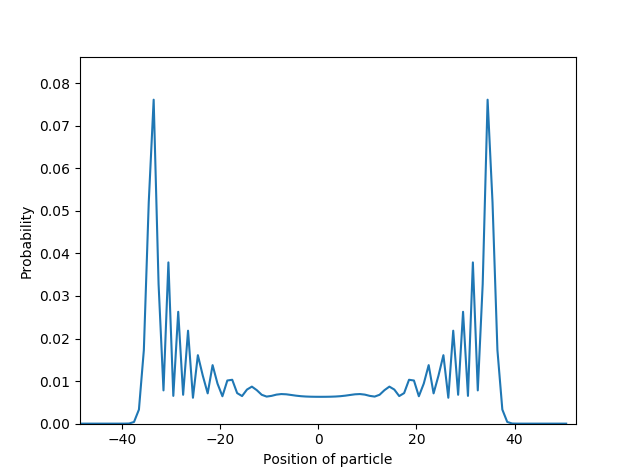
\includegraphics[scale=0.7]{1_Intro/Figures/coined_walk_results.png}
    \caption{Probability distribution of 100 steps DTQW using the above defined coined and translational operators}
    \label{fig:my_label}
\end{figure}
%%%%%%%%%%%%%%%%%%%%%
\textbf{Quantum Walks on a Graph \& Scattering Theory} \newline
In the context of my thesis, the concept of quantum walks on a \textit{graph} is necessary, particularly based on scattering theory as presented by Dr. Feldmann and Dr. Hillery \cite{FELDMAN2004277}. In this scenario, the walker is incident at a vertex or node of a graph with $n$ edges. The particle possesses a reflection and transmission amplitude corresponding to the particle behavior at entering or exiting a particular vertex. The basis states for the particle correspond to the \textit{momentum} on the edge. Therefore any operator acting in a graph with $n$ edges will have dimensions $2n$. \newline
Let $O$ be the vertex at which all the edges be meet, with the opposite ends of the edges labeled with numbers $1$ to $n$. Given any input state $\ket{kO}$ where $k$ is an integer from $1$ to $n$, the transition rule gives the amplitude to go to the output state $\ket{Ok}$ is given as $r$ and the amplitude for any other output state is $t$. Evolution is unitary under the beam splitter conditions of the following amplitudes:
\begin{equation}
    (n-1)|t|^2 + |r|^2 = 1
\end{equation}
\begin{equation}
    (n-2)|t|^2 + r^{*}t + t^{*}r = 0
\end{equation}
This approach allows for not needing a Hilbert space for the coin states which reduces the dimensionality of a system. 
\newpage
\section{Purpose of this Project}
The purpose of this thesis is to demonstrate the utilization of simple quantum simulations to model the physical phenomena of a complex physical system such as a molecular system. The molecular system in my thesis to be investigated is that of Benzene ($C_{6}H_{6}$). If a molecular system like Benzene can be modeled through optical quantum simulations, then such simulations can be scaled up to more complicated or larger molecules. Utilizing Benzene as a testing ground will allow us to understand the accuracy, efficiency, and limits of proposed methods. The benzene molecule will be modeled optically through an arrangement of directionally unbiased multiports (three-port in the context of this thesis). 
Running quantum simulations will be highly beneficial to the medical and pharmaceutical industry for its potential for creating complex models of how the human body functions or modeling the processes governing chemical reactions leading to faster drug discovery for complex diseases such as cancer. Benzene (aromatic hydrocarbon, component of crude oil and gasoline, and produced across the U.S. in plastics, resins, etc.) is a cause of acute myeloid leukemia and other malignancies \cite{doi:10.1093/carcin/bgr297}. Benzene is often used as a probe in identifying and characterizing binding pockets of proteins for structural design. Simulating the energy dynamics of benzene will allow researchers to learn more about the chemical processes governing benzene for designing better drugs or probes. If our proposed methods are successful then this will allow researchers to model other hydrocarbons or chemical systems such as Curcumin ($C_{21}H_{20}O_{6}$) which has anticancer benefits but hasn't been extensively studied and modeled yet \cite{article}. 

